%\subsection{Analysis starting from modulation/PER}
%\label{sec_phy_modulation}

In practice, it might not be possible to achieve perfect interference cancellation.
%Without considering partial interference cancellation and modulation, (\ref{eq_sic_shannon}) is too optimistic to evaluate the performance of NOMA with SIC. 
The authors in~\cite{cite_bell1} have show simulation results for SIC with respect to modulation schemes and SNR difference as given in Fig.~\ref{fig_NOMA_modulation}. All points enclosed in the upper right area of each curve are in the desired operating region with $\text{PER} \leq 10^{-2}.$  
Table~\ref{tb_NOMA_modulation} further shows the relationship between modulation and SNR for three marked points in the figure. We can find that the simulation result does not strictly follow (\ref{eq_sic_shannon}). For example, if the SNR of U1 becomes 8 times (i.e. 9 dB) larger, the modulation of U1 can upgrade from QPSK to 16QAM, which has only 2 times larger capacity. 
%
Fig.~\ref{fig_NOMA_modulation} motivates our further investigation on the practical performance of SIC for MAC layer design.
%Therefore, (\ref{eq_sic_shannon}) should be modified and we will analyze how to construct SNR-modulation model and equation in the future works.


\begin{figure}[t]
\begin{center}
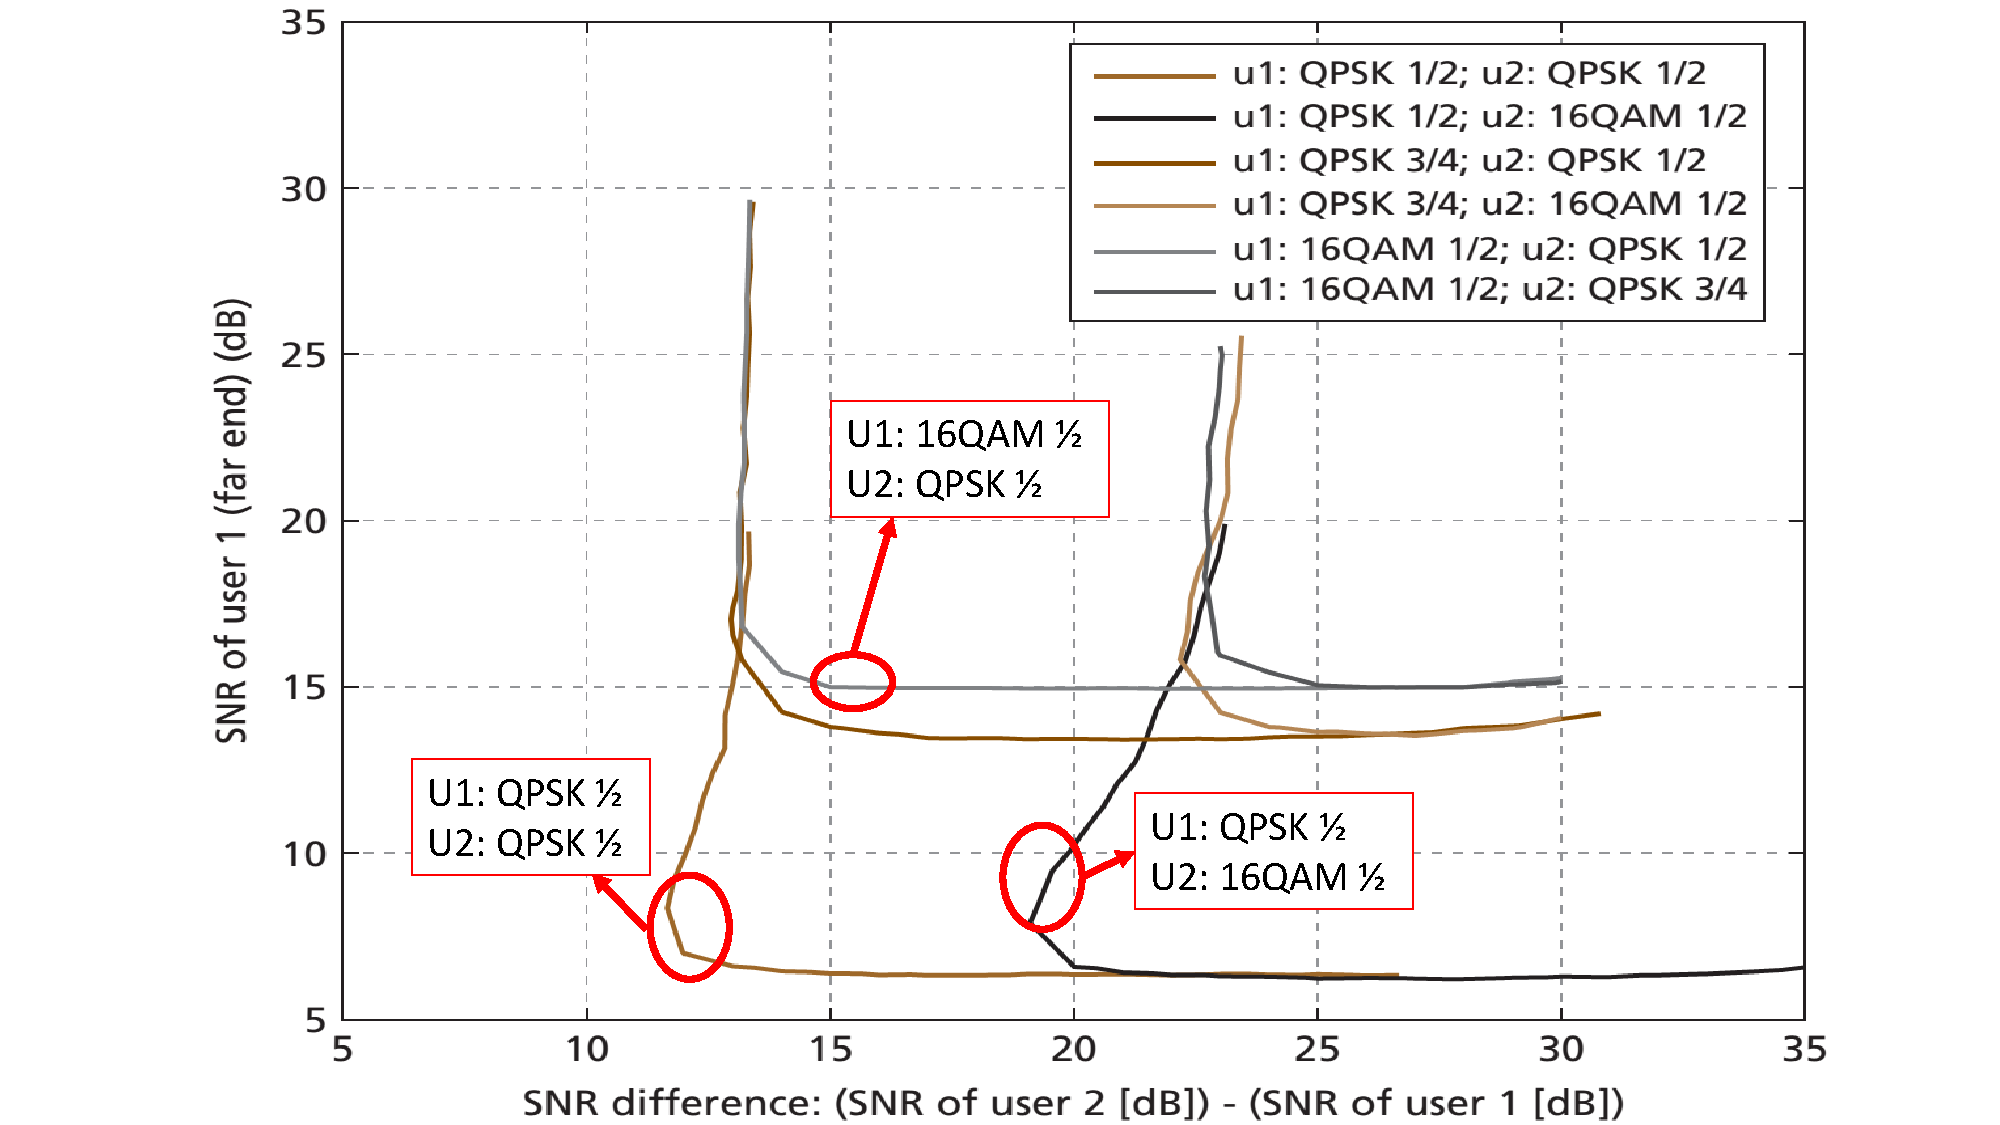
\includegraphics[width=1\columnwidth ,angle=0]{figure/NOMA_modulation}
\caption{Modulation and PER vs. SNR difference}
\label{fig_NOMA_modulation}
\end{center}
\end{figure}
%

\begin{table}[t]
\caption{Modulation curve in Fig.~\ref{fig_NOMA_modulation}}
    \begin{tabular}{| l | l | l | l |}
    \hline
    U1 Modulation & U2 Modulation & SNR of U1 & SNR Diff \\ \hline
    QPSK 1/2       & QPSK 1/2       & 6-15           & 12-20                  \\ \hline
    QPSK 1/2       & 16QAM 1/2     & 6-15           &  $\geq$ 20                     \\ \hline
    16QAM 1/2     & QPSK 1/2       & $\geq$15            & 12-20                   \\ \hline
    \end{tabular}
\label{tb_NOMA_modulation}
\end{table}